%; whizzy chapter -dvi
% -initex iniptex -latex platex -format platex -bibtex jbibtex -fmt fmt
% $B0J>e(B whizzytex $B$r;HMQ$9$k>l9g$N@_Dj!#(B
 
%     Tokyo Debian Meeting resources
%     Copyright (C) 2012 Junichi Uekawa
%     Copyright (C) 2011, 2015 Nobuhiro Iwamatsu

%     This program is free software; you can redistribute it and/or modify
%     it under the terms of the GNU General Public License as published by
%     the Free Software Foundation; either version 2 of the License, or
%     (at your option) any later version.

%     This program is distributed in the hope that it will be useful,
%     but WITHOUT ANY WARRANTY; without even the implied warranty of
%     MERCHANTABILITY or FITNESS FOR A PARTICULAR PURPOSE.  See the
%     GNU General Public License for more details.

%     You should have received a copy of the GNU General Public License
%     along with this program; if not, write to the Free Software
%     Foundation, Inc., 51 Franklin St, Fifth Floor, Boston, MA  02110-1301 USA

%  preview (shell-command (concat "evince " (replace-regexp-in-string "tex$" "pdf"(buffer-file-name)) "&"))

%%$B$3$3$+$i%X%C%@3+;O!#(B

\documentclass[mingoth,a4paper]{jsarticle}
\usepackage{monthlyreport}
% $BF|IU$rDj5A$9$k!"Kh7nJQ$o$j$^$9!#(B
\newcommand{\debmtgyear}{2017}
\newcommand{\debmtgmonth}{4}
\newcommand{\debmtgdate}{22}
% started from zero:
% (let ((year 2013) (month 7)) (+ (* (- year 2005) 12) month -1))
\newcommand{\debmtgnumber}{150}

% tikz picture $B$N0Y$N%^%/%m@_Dj(B
\usepackage[dvipdfmx]{graphicx}
\usepackage{tikz}

\begin{document}

\begin{titlepage}
\thispagestyle{empty}
% $B%?%$%H%k%Z!<%8(B:$BJT=8I,MW$JItJ,$O:G=i$N%^%/%m$KHt$P$9$3$H(B

\vspace*{-2cm}
$BBh(B\debmtgnumber{}$B2s(B $BEl5~%(%j%"(B Debian $BJY6/2q;qNA(B\\
\hspace*{-2cm}
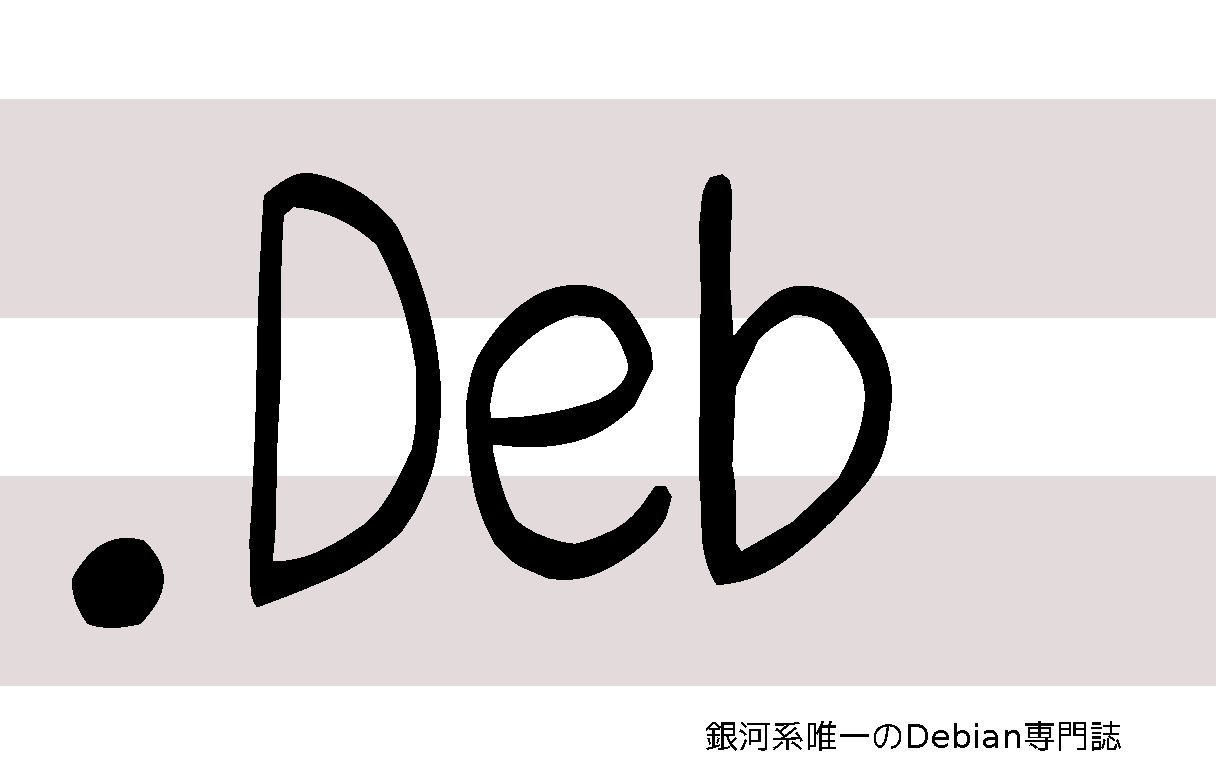
\includegraphics{image2012-natsu/dotdeb.pdf}\\
\hfill{}\debmtgyear{}$BG/(B\debmtgmonth{}$B7n(B\debmtgdate{}$BF|(B

% $B$3$3$O%"%C%W%G!<%H$9$k$3$H(B
% $BA43QJ8;z$K$7$J$$$H%U%)%s%H$N%5%$%:$,9g$o$J$$$N$GCm0U(B
\rotatebox{10}{\fontsize{30}{30} {\gt $BFC=8(B $B!'%Q%C%1!<%8%+%9%?%^%$%:(B}}\\

\vspace*{-2cm}
\hfill{}
\includegraphics[height=6cm]{image200502/openlogo-nd.eps}
\end{titlepage}

\newpage

\begin{minipage}[b]{0.2\hsize}
 \definecolor{titleback}{gray}{0.9}
 \colorbox{titleback}{\rotatebox{90}{\fontsize{80}{80} {\gt $B%G%S%"%sJY6/2q(B} }}
\end{minipage}
\begin{minipage}[b]{0.8\hsize}
\hrule
\vspace{2mm}
\hrule
\begin{multicols}{2}
\tableofcontents
\end{multicols}
\vspace{2mm}
\hrule
\end{minipage}

\dancersection{$B:G6a$N(BDebian$B4XO"$N%_!<%F%#%s%0Js9p(B}{$B?yK\(B $BE5=<(B}

\subsection{$BBh(B148$B2sEl5~%(%j%"(BDebian$BJY6/2q(B}

2017$BG/(B2$B7n(B11$BF|(B($BEZ(B)$B$KBh(B148$B2sEl5~%(%j%"(BDebian$BJY6/2q$r3+:E$7$^$7$?!#2q>l$O6d:B$K$"$kD+F|%M%C%H$5$s$r$*<Z$j$7$F9T$$$^$7$?!#;22C<T$O(B9$BL>$G$7$?!#(B

2017$BG/(B2$B7n(B5$BF|$K(BDebian 9 stretch$B$N(BFull Freeze$B@k8@$,%"%J%&%s%9$5$l$^$7$?(B\footnote{\url{https://lists.debian.org/debian-devel-announce/2017/02/msg00001.html}}$B!#:#2s$NJY6/2q$G$O!"%j%j!<%9%/%j%F%#%+%k%P%0$r2r7h$9$k$Y$/:n6H$r9T$&!V%P%0!&%9%+%C%7%e!&%Q!<%F%#!<!W$r9T$$$^$7$?!#(B

Debian Developer$B$G$"$k4d>>$5$s$+$i%j%j!<%9%/%j%F%#%+%k%P%0$ND4$YJ}!"(Bpatch$B$NEj9F:nK!!"(BBTS$B$X$N%?%0$N8z2LE*$J$D$1J}$r;22C<T$X6&M-$7$^$7$?!#$=$N8e!"%j%j!<%9%/%j%F%#%+%k%P%0$NCf$GFq0WEY$N9b$$$b$N$HDc$$$b$N$rA*JL$7!";22C<T$O2r7h$G$-$k$b$N$+$i%P%02r7h$KNW$_$^$7$?!#(B

$B%P%0!&%9%+%C%7%e!&%Q!<%F%#$N7k2L$O!"0J2<$N(BDebian wiki$B$K$^$H$a$F$$$^$9!#(B

\url{https://wiki.debian.org/BSP/2017/02/jp/Tokyo}


\subsection{OSC 2017 Tokyo/Spring $B=PE8!JBh(B149$B2sEl5~%(%j%"(BDebian$BJY6/2q!K(B}

2017$BG/(B3$B7n(B11$BF|(B($BEZ(B)$B$K3+:E$5$l$?(BOSC 2017 Tokyo/Spring$B$X!"El5~%(%j%"(BDebian$BJY6/2q(B/DebianJP$B$H$7$F=PE8$7$^$7$?!#(B

$BE8<(%V!<%9$G$O(BDebian GNU/Linux$B$r%$%s%9%H!<%k$7$?(BPC$B5Z$S(BARM$B$H(BFPGA$B$NN>J}$rEk:\$7$?%j%U%!%l%s%9%\!<%I$NE8<(!"(BDebian Project$B$HEl5~%(%j%"(BDebian$BJY6/2q$N9-Js3hF0$r9T$$$^$7$?!#$^$?!"(BOSC$B;22C<T$H8rN.$r?<$a$^$7$?!#(B

$B%;%_%J!<$O!VBh(B149$B2sEl5~%(%j%"(BDebian$BJY6/2q!W$H$7$F3+:E$7!"!V(BDebian updates$B!W$H$$$&I=Bj$G4d>>$5$s$,H/I=$7$^$7$?!#$^$?!"%;%_%J!<$K;22C$7$?(B25$BL>$NJ}!9$+$i5?Ld$d<ALd$K2sEz$7$^$7$?!#(B


\dancersection{$B;vA02]Bj(B}{$B?yK\(B $BE5=<(B}

$B:#2s$N;vA02]Bj$O0J2<$G$9(B:
\begin{enumerate}
  \item Hack Time$B$O2?$r$7$^$9$+!#(B
  \item $BIaCJ;H$C$F$$$k(BDebian$B%Q%C%1!<%8$N$&$A!"%+%9%?%^%$%:!J%3%s%Q%$%k%*%W%7%g%sJQ99$dFH<+=$@5$J$I!K$7$F$$$k$b$N$,$"$l$P!"$=$N%Q%C%1!<%8L>$H%+%9%?%^%$%:FbMF$r=q$$$F$/$@$5$$!#(B
\end{enumerate}
$B$3$N2]Bj$KBP$7$FDs=P$$$?$@$$$?FbMF$O0J2<$G$9!#(B
\begin{multicols}{2}
{\small
\begin{prework}{ user }
  \begin{enumerate}
  \item aaa
  \end{enumerate}
\end{prework}

}
\end{multicols}

\dancersection{Debian Trivia Quiz}{$B?yK\(B $BE5=<(B}

Debian$B$N:r:#$NOCBj$K$D$$$F$N(BQuiz$B$G$9!#(B

$B:#2s$N=PBjHO0O$O(B\url{debian-devel-announce@lists.debian.org} $B$d(B \url{debian-news@lists.debian.org}$B$J$I$KEj9F$5$l$?FbMF$+$i$G$9!#(B

\begin{multicols}{2}
%; whizzy-master ../debianmeetingresume201311.tex
% $B0J>e$N@_Dj$r$7$F$$$k$?$a!"$3$N%U%!%$%k$G(B M-x whizzytex $B$9$k$H!"(Bwhizzytex$B$,MxMQ$G$-$^$9!#(B
%

\santaku
{2017$BG/$N(BDebian Project Leader(=DPL)$BA*5s$,9T$o$l!"EjI<7k2L$,H/I=$5$l$^$7$?!#(BDPL$B$KA*$P$l$?$N$OC/$G$7$g$&$+!#(B}
{Mehdi Dogguy}
{Nobuhiro Iwamatsu}
{Chris Lamb}
{C}
{Chris Lamb$B$5$s$,A*=P$5$l$^$7$?!#$*$a$G$H$&$4$6$$$^$9!*(B\url{https://bits.debian.org/2017/04/results-dpl-elections-2017.html}$B!#$J$*!"(B2017$BG/(BDPL$BA*5s$N>pJs$O<!$N(Bweb$B%Z!<%8$r;2>H$/$@$5$$(B\url{https://www.debian.org/vote/2017/vote_001}$B!#(B}

\end{multicols}


% % (query-replace-regexp "<.*?>" "")
% % (query-replace-regexp "^[	 ]\+" "")

%-------------------------------------------------------------------------------
\dancersection{Debian$B%Q%C%1!<%8$N%+%9%?%^%$%:$K$D$$$F(B}{yy\_y\_ja\_jp}
%-------------------------------------------------------------------------------

\subsection{$B$O$8$a$K(B}

Debian$B%Q%C%1!<%8$r%+%9%?%^%$%:$7$?$$$1$I$d$jJ}$,!JFC$K$I$3$K=q$$$F$"$k$N$+!K(B
$BJ,$+$i$J$$$H$$$&OC$,$"$C$?$N$G!"$^$H$a$F$_$^$7$?!#(B

$B$^$:%Q%C%1!<%8%s%0$NA0Ds$r8+$F$$$-$^$9!#(B

$B<!$K!"%+%9%?%^%$%:$7$?$$>l=j$OBg$-$/(B2$B$D$"$k$G$7$g$&!#(B

\begin{itemize}
 \item Debian$B%Q%C%1!<%8%s%0$NItJ,(B
 \item $B>eN.$N%3!<%I<+BN(B
\end{itemize}

$B$^$?!"$3$l$i%+%9%?%^%$%:$7$?FbMF$r$=$N8e%a%s%F%J%s%9$7$F$$$/I,MW$,$"$j$^$9!#(B

$B$=$l$>$l8+$F$$$-$^$7$g$&!#(B

\subsection{$BA0Ds(B}
$B%Q%C%1!<%8%s%0$K$D$$$F$N35MW$O(B``$B%Q%C%1!<%8%s%0%A%e!<%H%j%"%k(B''$B$K$"$k$N$G(B
\verb|apt install packaging-tutorial|$B$r<B9T$7$F$+$i(B
\verb|/usr/share/doc/packaging-tutorial/|$B$NCf$r8+$F$_$^$7$g$&(B
\footnote{\url{https://www.debian.org/doc/manuals/packaging-tutorial/packaging-tutorial.ja.pdf}
$B$K$b$"$j$^$9!#(B}$B!#(B

$B%+%9%?%^%$%:$9$k$K$O%Q%C%1!<%8$N%=!<%9%3!<%I$r<j85$KMQ0U$9$kI,MW$,(B
$B$"$j$^$9!#(B\verb|apt-get source|$B$d(Bdget(1)$B!J(Bdevscripts$B%Q%C%1!<%8$K(B
$B$"$j$^$9!K$G%@%&%s%m!<%I$G$-$^$9!#(B
$B%a%s%F%J$,%Q%C%1!<%8%s%0:n6HMQ$N(Bgit$B%l%]%8%H%j$J$I$r8x3+$7$F$$$k>l9g(B
$B!J(B\verb|Vcs-*|$B%U%#!<%k%I!K$O!"(Bdebcheckout(1)$B!J(Bdevscripts$B%Q%C%1!<%8!K$b;H$&$H$=(B
$B$N%l%]%8%H%j$r(Bclone$B$7$?$j$7$F$/$l$k$h$&$G$9!#(B

$B$=$7$F!"(BDebian$B%Q%C%1!<%8$O(B ``Debian$B%]%j%7!<(B''$B!J(Bdebian-policy$B%Q%C%1!<%8!K(B
$B$K=>$C$F:n$i$l$F$$$^$9!#(B
Debian$B%]%j%7!<$O!"(BDebian$B$,$&$^$/F0$/$h$&$KDj$a$i$l$?%k!<%k$G$9!#(B
$B%+%9%?%^%$%:$7$?%Q%C%1!<%8$b%]%j%7!<$K=>$C$?$[$&$,$h$$$G$7$g$&!#(B
$BK\Ev$O%]%j%7!<A4J8$rFI$`$H$h$$$G$7$g$&!"$H8@$$$?$$$H$3$m$G$9$,D9J8$G$9!#(B
$B$^$?!"(BDebian$B%]%j%7!<0J30$K$b=>$C$F$*$$$?$[$&$,$h$$47=,$,(B ``Debian $B3+H/<T(B
$B%j%U%!%l%s%9(B''$B!J(Bdevelopers-reference-ja$B%Q%C%1!<%8!K(B
\footnote{\url{https://www.debian.org/doc/manuals/developers-reference/index.ja.html}
$B$K$b$"$j$^$9!#(B}$B$J$I$$$/$D$+$K=q$+$l$F$$$^$9!#(B

debhelper$B$J$I$N%Q%C%1!<%8%s%0%X%k%Q!<$O%]%j%7!<$K$G$-$k$@$1<+F0E*$K=>$C(B
$B$F%Q%C%1!<%8$,:n$i$l$k$h$&$K;EAH$s$G$"$j$^$9!#$J$N$GIaDL$K%Q%C%1!<%8%s%0%X%k%Q!<(B
$B$r;H$C$F%Q%C%1!<%8%s%0:n6H$r$7$F$$$l$P$"$kDxEY$O%]%j%7!<$K>!<j$K=>$C$F$$(B
$B$k$O$:$G$9!#(B

$B$^$?!"(Blintian(1)$B$H$$$&%D!<%k!J(Blintian$B%Q%C%1!<%8!K$,(BDebian$B%]%j%7!<$K0cH?$7$F$$$J$$$+!"47=,$K1h$C$F$$(B
$B$k$+%A%'%C%/$7$F$/$l$^$9!#(Blintian$B$O%$%s%9%H!<%k:Q$_$J$i%Q%C%1!<%8%s%0%3(B
$B%^%s%I(Bdebuild$B$N:G8e$G<+F0E*$K8F$P$l$^$9!#(B
$B<B:]$N$H$3$m$$$m$s$J47=,$,$$$m$s$J>l=j$K=q$$$F(B
$B$"$C$F$o$+$i$J$$$3$H$bB?$$$N$G!"$^$:$O:n$C$?%Q%C%1!<%8$r(Bdebuild$B$7$F$_$F!"(B
lintian$B$N7k2L$r8+$F!"%(%i!<$d7Y9p$,=P$?$i>\:Y@bL@$rFI$s$G=$@5$7$^$7$g$&!#(B

$BFC$K!"47=,$N(B1$B$D$K$O%P!<%8%g%sHV9f$,$"$j$^$9!#3+H/<T%l%U%!%l%s%9$K$h$k$H!"(B
$B%Q%C%1!<%8%a%s%F%J0J30$,%Q%C%1!<%8$rJQ99$7$F(BDebian$BK\BN$K%"%C%W%m!<%I$9$k(B
$B$H$-(B(Non-Maintainer Upload, NMU)$B$K(B
$B$O!"JQ99FbMF$r(B debian/changelog $B$K=q$-!"FCJL$J%P!<%8%g%sHV9f$K$7$J$1$l$P$J$j$^$;$s!#(B
$B>o$K%a%s%F%J$N%"%C%W%m!<%I$9$k%P!<%8%g%s$,M%@h$5$l$k$h$&$K!"<!$K%a%s%F%J(B
$B$,%"%C%W%m!<%I$9$k$G$"$m$&%P!<%8%g%sHV9f$h$j$bDc$/$7$F$$$k$+$i$G$9!#(B
$BK\Ev$K(BNMU$B$9$k$o$1$G$O$J$$$K$;$h=EMW$J$N$G!"$3$l$K$D$$$F$O0J9_$b8+$F$$$-$^$9!#(B

\subsection{Debian$B%Q%C%1!<%8%s%0$NItJ,(B\label{sec:customize-debpkg}}

$B$3$l$K$D$$$F$O(B

\begin{itemize}
 \item $B%3%s%Q%$%k%*%W%7%g%s$J$I$rJQ99$7$?$$(B
 \item $B0MB84X78$d%Q%C%1!<%89=@.$J$I$rJQ99$7$?$$(B
 \item $BIT0BDjHG(B(unstable)$B$K$"$k%P!<%8%g%s$r0BDjHG(B(stable)$B$J$I$K%P%C%/%]!<%H$7$?$$(B
\end{itemize}

$B$J$I$,$"$k$G$7$g$&!#(B

\subsubsection{$B%3%s%Q%$%k%*%W%7%g%s(B}

$B%Q%C%1!<%8%s%0$G$O(B debian/rules $B%U%!%$%k$+$i%3%s%Q%$%k$,<B9T$5$l$^$9!#(B
$B%3%s%Q%$%k%*%W%7%g%s$rJQ99$9$k$H$-$O!"$3$l$rJQ99$9$k$@$1$N$3$H$,B?$$$G$9(B
$B!J@53N$K$O!"0lDL$jJQ99$7$F!"$=$NJQ99FbMF$r(B dch(1) $B%3%^%s%I$G(B
debian/changelog $B%U%!%$%k$K?7$7$$%P!<%8%g%sHV9f$G5-F~$7$?$i40@.$G$9!#0J(B
$B9_$bF1MM$G$9!K!#(B

$B$3$3$G$ONc$H$7$F(B hello $B$H$$$&%Q%C%1!<%8$r8+$F$_$^$9!#(B

\begin{commandline}
$ apt-get source hello
$B%Q%C%1!<%8%j%9%H$rFI$_9~$s$G$$$^$9(B... $B40N;(B
733 kB $B$N%=!<%9%"!<%+%$%V$r<hF@$9$kI,MW$,$"$j$^$9!#(B
$B<hF@(B:1 http://ftp.jp.debian.org/debian sid/main hello 2.10-1 (dsc) [1,323 B]
$B<hF@(B:2 http://ftp.jp.debian.org/debian sid/main hello 2.10-1 (tar) [726 kB]
$B<hF@(B:3 http://ftp.jp.debian.org/debian sid/main hello 2.10-1 (diff) [6,072 B]
733 kB $B$r(B 0$BIC(B $B$G<hF@$7$^$7$?(B (938 kB/s)
dpkg-source: info: extracting hello in hello-2.10
dpkg-source: info: unpacking hello_2.10.orig.tar.gz
dpkg-source: info: unpacking hello_2.10-1.debian.tar.xz
$ cd hello-2.10/
\end{commandline}

\begin{commandline}
$ editor debian/rules
\end{commandline}
\begin{commandline}
#!/usr/bin/make -f
%:
	dh $@

override_dh_auto_clean:
	[ ! -f Makefile ] || $(MAKE) distclean

override_dh_installdocs:
	dh_installdocs NEWS
\end{commandline}

$B$3$N(Bhello$B$K$O$"$^$jLLGr$=$&$J%*%W%7%g%s$,8+Ev$?$i$J$$$N$G$9$,!"$H$j$"$($:(B \verb|./configure| $B$K(B
\verb|--disable-nls|$B$rIU$1$F$_$^$9!#$5$F!"$I$3$K=q$1$P$$$$$+$o$+$i$J$$$N(B
$B$G$H$j$"$($:(Bdebuild$B$7$F$_$^$9!#(B

\begin{commandline}
$ debuild -us -uc
 dpkg-buildpackage -rfakeroot -us -uc
dpkg-buildpackage: info: source package hello
dpkg-buildpackage: info: source version 2.10-1
dpkg-buildpackage: info: source distribution unstable
(snip)
 debian/rules build
dh build
   dh_testdir
   dh_update_autotools_config
   dh_auto_configure
	./configure --build=x86_64-linux-gnu --prefix=/usr --includedir=\${prefix}/include --mandir=\${prefix}/share/man --infodir=\${prefix}/share/info --sysconfdir=/etc --localstatedir=/var --disable-silent-rules --libdir=\${prefix}/lib/x86_64-linux-gnu --libexecdir=\${prefix}/lib/x86_64-linux-gnu --disable-maintainer-mode --disable-dependency-tracking
configure: WARNING: unrecognized options: --disable-maintainer-mode
(snip)
\end{commandline}

$B$I$&$d$i(B\verb|dh_auto_configure|$B$K%*%W%7%g%s$rEO$;$P$$$$$h$&$J$N$G$=$&$7$F$_$^$9!#(B

\begin{commandline}
#!/usr/bin/make -f
%:
	dh $@

override_dh_auto_clean:
	[ ! -f Makefile ] || $(MAKE) distclean

override_dh_installdocs:
	dh_installdocs NEWS

override_dh_auto_configure:
	dh_auto_configure -- --disable-nls
\end{commandline}

debian/changelog $B$r=q$-$^$9!#(B\verb|dch|$B$r<B9T$9$k$H(B\footnote{$B<B9TA0$K(B
\texttt{DEBFULLNAME}, \texttt{DEBEMAIL} $B4D6-JQ?t$r@_Dj$7$F$/$@$5$$!#>\$7$/$O(B``$B?7%a%s%F%J!<%,%$%I(B''$B!J8e=R!K$K$"$j$^$9!#(B}$B!"%a%s%F%J$G$O$J$$$?(B
$B$a<+F0E*$K(B\verb|--nmu|$B%b!<%I$K$J$j$^$9!#%G%#%9%H%j%S%e!<%7%g%s$,(B
\verb|UNRELEASED|$B$K2>$G=q$+$l$^$9!#(B

\begin{commandline}
$ dch
$ head -n 10 debian/changelog
hello (2.10-1.1) UNRELEASED; urgency=medium

  * Non-maintainer upload.
  * debian/rules: Use --disable-nls.

 -- YOSHINO Yoshihito <yy.y.ja.jp@gmail.com>  Sat, 22 Apr 2017 08:58:38 +0900

hello (2.10-1) unstable; urgency=low

  * New upstream release.
\end{commandline}

$B$H$j$"$($:(B debuild $B$7$F$_$^$9!#:G8e$K(Blintian$B$,<B9T$5$l$F$k$N$G8+$^$7$g$&!#(B

\begin{commandline}
$ debuild -us -uc
 dpkg-buildpackage -rfakeroot -us -uc
dpkg-buildpackage: info: source package hello
dpkg-buildpackage: info: source version 2.10-1.1
dpkg-buildpackage: info: source distribution unstable
(snip)
   dh_md5sums
   dh_builddeb
dpkg-deb: building package 'hello-dbgsym' in '../hello-dbgsym_2.10-1.1_amd64.deb'.
dpkg-deb: building package 'hello' in '../hello_2.10-1.1_amd64.deb'.
 dpkg-genbuildinfo
 dpkg-genchanges  >../hello_2.10-1.1_amd64.changes
dpkg-genchanges: info: not including original source code in upload
 dpkg-source --after-build hello-2.10
dpkg-buildpackage: info: binary and diff upload (original source NOT included)
Now running lintian...
W: hello source: ancient-standards-version 3.9.6 (current is 3.9.8)
Finished running lintian.
\end{commandline}

lintian$B$N3F9T$N>\:Y@bL@$O(B lintian-info(1) $B$G8+$i$l$^$9(B
\footnote{\url{https://lintian.debian.org/tags/ancient-standards-version.html}
$B$G$b8+$i$l$^$9$,!"LdBj$N$"$kA4%Q%C%1!<%8$,:\$C$F$$$k$N$G=E$$$G$9!#(B}$B!#(B

\begin{commandline}
$ lintian-info --tags ancient-standards-version
W: ancient-standards-version
N:
N:   The source package refers to a Standards-Version that has been
N:   obsolete for more than two years. Please update your package to latest
N:   Policy and set this control field appropriately.
N:   
N:   If the package is already compliant with the current standards, you
N:   don't have to re-upload the package just to adjust the
N:   Standards-Version control field. However, please remember to update
N:   this field next time you upload the package.
N:   
N:   See /usr/share/doc/debian-policy/upgrading-checklist.txt.gz in the
N:   debian-policy package for a summary of changes in newer versions of
N:   Policy.
N:   
N:   Refer to https://www.debian.org/doc/debian-policy/upgrading-checklist
N:   for details.
N:   
N:   Severity: normal, Certainty: certain
N:   
N:   Check: standards-version, Type: source
N:
\end{commandline}

$B$J$*!"$3$NNc$G$O%+%9%?%^%$%:$9$kA0$+$i(B\verb|ancient-standards-version|$B$,(B
$B=P$F$$$k$h$&$J$N$G!"=$@5$;$:$=$N$^$^$K$7$F$*$-$^$9!#%a%s%F%J$,<!$K%j%j!<%9$7$?$H(B
$B$-$KD>$9$G$7$g$&$7!"$=$l$KBP$7$F<+J,$N%+%9%?%^%$%:$r$7$?$$$H$-$K!"<+J,$N(B
$B%+%9%?%^%$%:FbMF$@$1$rJQ99$9$l$P$h$$$+$i$G$9!#(B

$B%+%9%?%^%$%:$,40N;$7$?$i%G%#%9%H%j%S%e!<%7%g%s$r3NDj$5$;$^$9!#(B
$B0J2<$r<B9T$7$F%(%G%#%?$GJ]B8$7$^$9!#(B

\begin{commandline}
$ dch -r
$ head -n 10 debian/changelog
hello (2.10-1.1) unstable; urgency=medium

  * Non-maintainer upload.
  * debian/rules: Use --disable-nls.

 -- YOSHINO Yoshihito <yy.y.ja.jp@gmail.com>  Sat, 22 Apr 2017 09:00:30 +0900

hello (2.10-1) unstable; urgency=low

  * New upstream release.
\end{commandline}

debuild $B$9$l$P40@.$G$9!#(B

\begin{commandline}
$ debuild -us -uc
 dpkg-buildpackage -rfakeroot -us -uc
dpkg-buildpackage: info: source package hello
dpkg-buildpackage: info: source version 2.10-1.1
dpkg-buildpackage: info: source distribution unstable
(snip)
   dh_md5sums
   dh_builddeb
dpkg-deb: building package 'hello-dbgsym' in '../hello-dbgsym_2.10-1.1_amd64.deb'.
dpkg-deb: building package 'hello' in '../hello_2.10-1.1_amd64.deb'.
 dpkg-genbuildinfo
 dpkg-genchanges  >../hello_2.10-1.1_amd64.changes
dpkg-genchanges: info: not including original source code in upload
 dpkg-source --after-build hello-2.10
dpkg-buildpackage: info: binary and diff upload (original source NOT included)
Now running lintian...
W: hello source: ancient-standards-version 3.9.6 (current is 3.9.8)
Finished running lintian.
\end{commandline}

$B$5$F!"$3$3$^$G!J(B\verb|dch|$B$H0z?t$J$7$G5/F0$9$k$3$H$G!K(BNMU$B$9$k%Q%C%1!<%8%s%0:n6H$r(B
$B$7$F$-$^$7$?!#(BDebian$BK\BN$K%"%C%W%m!<%I$9$k$N$G$O$J$/8D?ME*$K;H$C$?$j$9$k(B
$B$?$a$N%+%9%?%^%$%:$G$"$l$P!"(BNMU$B$G$O$J$/(B``$B%m!<%+%k%"%C%W%m!<%I(B''$B$K$7$?$[(B
$B$&$,$h$$$G$7$g$&!#%m!<%+%k%"%C%W%m!<%I$K$OL>A0$rIU$1$^$9!#$3$3$G$OL>A0$r(Bysn$B$K(B
$B$7$F$_$^$9!#(B

\begin{commandline}
$ dch --local ysn
\end{commandline}

\begin{commandline}
$ head -n 10 debian/changelog
hello (2.10-1ysn1) UNRELEASED; urgency=medium

  * debian/rules: Use --disable-nls.

 -- YOSHINO Yoshihito <yy.y.ja.jp@gmail.com>  Sat, 22 Apr 2017 08:44:10 +0900

hello (2.10-1) unstable; urgency=low

  * New upstream release.
  * debian/patches: Drop 01-fix-i18n-of-default-message, no longer needed.
(snip)
\end{commandline}

debuild $B$7$F$_$^$9!#(B

\begin{commandline}
$ debuild -us -uc
 dpkg-buildpackage -rfakeroot -us -uc
dpkg-buildpackage: info: source package hello
dpkg-buildpackage: info: source version 2.10-1ysn1
dpkg-buildpackage: info: source distribution UNRELEASED
(snip)
   dh_md5sums
   dh_builddeb
dpkg-deb: building package 'hello-dbgsym' in '../hello-dbgsym_2.10-1ysn1_amd64.deb'.
dpkg-deb: building package 'hello' in '../hello_2.10-1ysn1_amd64.deb'.
 dpkg-genbuildinfo
 dpkg-genchanges  >../hello_2.10-1ysn1_amd64.changes
dpkg-genchanges: info: not including original source code in upload
 dpkg-source --after-build hello-2.10
dpkg-buildpackage: info: binary and diff upload (original source NOT included)
Now running lintian...
W: hello source: changelog-should-mention-nmu
W: hello source: source-nmu-has-incorrect-version-number 2.10-1ysn1
W: hello source: ancient-standards-version 3.9.6 (current is 3.9.8)
Finished running lintian.
\end{commandline}

lintian$B$,7Y9p$7$F$$$k$h$&$J$N$G8+$F$_$^$9!#(B

\begin{commandline}
$ lintian-info --tags changelog-should-mention-nmu source-nmu-has-incorrect-version-number
W: changelog-should-mention-nmu
N:
N:   When you NMU a package, that fact should be mentioned on the first
N:   line in the changelog entry. Use the words "NMU" or "Non-maintainer
N:   upload" (case insensitive).
N:   
N:   Maybe you didn't intend this upload to be a NMU, in that case, please
N:   double-check that the most recent entry in the changelog is
N:   byte-for-byte identical to the maintainer or one of the uploaders. If
N:   this is a local package (not intended for Debian), you can suppress
N:   this warning by putting "local" in the version number or "local
N:   package" on the first line of the changelog entry.
N:   
N:   Refer to Debian Developer's Reference section 5.11.3 (Using the
N:   DELAYED/ queue) for details.
N:   
N:   Severity: normal, Certainty: certain
N:   
N:   Check: nmu, Type: source
N:
\end{commandline}
\begin{commandline}
W: source-nmu-has-incorrect-version-number
N:
N:   A source NMU should have a Debian revision of "-x.x" (or "+nmuX" for a
N:   native package). This is to prevent stealing version numbers from the
N:   maintainer.
N:   
N:   Maybe you didn't intend this upload to be a NMU, in that case, please
N:   double-check that the most recent entry in the changelog is
N:   byte-for-byte identical to the maintainer or one of the uploaders. If
N:   this is a local package (not intended for Debian), you can suppress
N:   this warning by putting "local" in the version number or "local
N:   package" on the first line of the changelog entry.
N:   
N:   Refer to Debian Developer's Reference section 5.11.2 (NMUs and
N:   debian/changelog) for details.
N:   
N:   Severity: normal, Certainty: certain
N:   
N:   Check: nmu, Type: source
N:
\end{commandline}

Debian $B$K%"%C%W%m!<%I$9$kL\E*$N%Q%C%1!<%8$G$O$J$$$N$G!"(Bdebian/changelog$B$r=$@5$7$^$9!#(B

\begin{commandline}
$ dch
$ head -n 10 debian/changelog
hello (2.10-1ysn1) UNRELEASED; urgency=medium

  * Local package.
  * debian/rules: Use --disable-nls.

 -- YOSHINO Yoshihito <yy.y.ja.jp@gmail.com>  Sat, 22 Apr 2017 08:44:10 +0900

hello (2.10-1) unstable; urgency=low

  * New upstream release.
\end{commandline}

$B$3$3$G$O(B \verb|Local package|$B$H=q$/$3$H$K$7$^$7$?$,!"(B
\verb|dch --local local|$B$G$b$$$$$G$7$g$&!#(B
debuild $B$7$^$9!#(B

\begin{commandline}
$ debuild -us -uc
 dpkg-buildpackage -rfakeroot -us -uc
dpkg-buildpackage: info: source package hello
dpkg-buildpackage: info: source version 2.10-1ysn1
dpkg-buildpackage: info: source distribution UNRELEASED
(snip)
   dh_md5sums
   dh_builddeb
dpkg-deb: building package 'hello-dbgsym' in '../hello-dbgsym_2.10-1ysn1_amd64.deb'.
dpkg-deb: building package 'hello' in '../hello_2.10-1ysn1_amd64.deb'.
 dpkg-genbuildinfo
 dpkg-genchanges  >../hello_2.10-1ysn1_amd64.changes
dpkg-genchanges: info: not including original source code in upload
 dpkg-source --after-build hello-2.10
dpkg-buildpackage: info: binary and diff upload (original source NOT included)
Now running lintian...
W: hello source: ancient-standards-version 3.9.6 (current is 3.9.8)
Finished running lintian.
\end{commandline}

$BLdBj$J$5$=$&$J$N$G(B\verb|dch -r|$B$7$F(Bdebuild$B$9$l$P40@.$G$9!#(B

\subsubsection{$B0MB84X78!&%Q%C%1!<%89=@.(B}

$B0MB84X78$d%Q%C%1!<%89=@.$O(B debian/control $B$K=q$+$l$F$$$k$N$G!"JQ99$9$k$J(B
$B$i$3$l$rJQ99$9$k$@$1$G$9!#(B

\subsubsection{$B%P%C%/%]!<%H(B}

$B%P%C%/%]!<%H$9$k:]$K$O!"4pK\E*$K$O(B \verb|dch --bpo| $B$9$k$@$1$G!"B>$N>l=j$OJQ99(B
$B$7$F$O$$$1$^$;$s!#%P%C%/%]!<%H@h$N%i%$%V%i%j$N%P!<%8%g%s$,8E$$$H$-$O(B
debian/control $B$N0MB84X78$rJQ99$9$kI,MW$,$"$k$3$H$,$"$j$^$9!#(B

jessie $B$K%P%C%/%]!<%H$7$F$_$^$9!#(B

\begin{commandline}
$ apt-get source hello
(snip)
$ cd hello-2.10/
$ dch --bpo
\end{commandline}

\verb|  * | $B$@$1$N9T$,<+F0E*$KDI2C$5$l$^$9$,!":#2s$OFC$K0MB84X78$OJQ$($F$J$$$N$G:o=|$7$FJ]B8$7$^$9!#(B

\begin{commandline}
$ head -n 10 debian/changelog
hello (2.10-1~bpo8+1) jessie-backports; urgency=medium

  * Rebuild for jessie-backports.

 -- YOSHINO Yoshihito <yy.y.ja.jp@gmail.com>  Sat, 22 Apr 2017 09:09:11 +0900

hello (2.10-1) unstable; urgency=low

  * New upstream release.
  * debian/patches: Drop 01-fix-i18n-of-default-message, no longer needed.
\end{commandline}

debuild $B$7$F$_$^$9!#(B

\begin{commandline}
$ debuild -us -uc
 dpkg-buildpackage -rfakeroot -us -uc
dpkg-buildpackage: info: source package hello
dpkg-buildpackage: info: source version 2.10-1~bpo8+1
dpkg-buildpackage: info: source distribution jessie-backports
(snip)
   dh_md5sums
   dh_builddeb
dpkg-deb: building package 'hello-dbgsym' in '../hello-dbgsym_2.10-1~bpo8+1_amd64.deb'.
dpkg-deb: building package 'hello' in '../hello_2.10-1~bpo8+1_amd64.deb'.
 dpkg-genbuildinfo
 dpkg-genchanges  >../hello_2.10-1~bpo8+1_amd64.changes
dpkg-genchanges: info: not including original source code in upload
 dpkg-source --after-build hello-2.10
dpkg-buildpackage: info: binary and diff upload (original source NOT included)
Now running lintian...
W: hello source: changelog-should-mention-nmu
W: hello source: source-nmu-has-incorrect-version-number 2.10-1~bpo8+1
W: hello source: ancient-standards-version 3.9.6 (current is 3.9.8)
Finished running lintian.
\end{commandline}

lintian $B$K=>$C$F=$@5$7$F$_$^$9!#(B

\begin{commandline}
$ dch
$ head -n 10 debian/changelog
hello (2.10-1~bpo8+1) jessie-backports; urgency=medium

  * Local package.
  * Rebuild for jessie-backports.

 -- YOSHINO Yoshihito <yy.y.ja.jp@gmail.com>  Sat, 22 Apr 2017 09:09:11 +0900

hello (2.10-1) unstable; urgency=low

  * New upstream release.
$ debuild -us -uc
 dpkg-buildpackage -rfakeroot -us -uc
dpkg-buildpackage: info: source package hello
dpkg-buildpackage: info: source version 2.10-1~bpo8+1
dpkg-buildpackage: info: source distribution jessie-backports
(snip)
 dpkg-genchanges  >../hello_2.10-1~bpo8+1_amd64.changes
dpkg-genchanges: info: not including original source code in upload
 dpkg-source --after-build hello-2.10
dpkg-buildpackage: info: binary and diff upload (original source NOT included)
Now running lintian...
W: hello source: ancient-standards-version 3.9.6 (current is 3.9.8)
Finished running lintian.
\end{commandline}

$B$H$j$"$($:2r>C$7$^$7$?!#$G$9$,!"8D?ME*$K$O(BDebian$B$G8x<0$J%P%C%/%]!<%H$,%j(B
$B%j!<%9$5$l$?$i99?7$5$l$F$[$7$$$N$G$A$g$C$HITK~$G$9!#(Blintian $B%(%i!<$O$&$^$/(B
$B>C$($J$$$N$G$9$,!">/$7%P!<%8%g%sHV9f$r2<$2$F;H$&$3$H$K$7$F$$$^$9!#(B

\begin{commandline}
$ head -n 10 debian/changelog
hello (2.10-1~bpo8+0.1) jessie-backports; urgency=medium

  * Local package.
  * Rebuild for jessie-backports.

 -- YOSHINO Yoshihito <yy.y.ja.jp@gmail.com>  Sat, 22 Apr 2017 09:09:11 +0900

hello (2.10-1) unstable; urgency=low

  * New upstream release.
\end{commandline}
\begin{commandline}
$ debuild -us -uc
 dpkg-buildpackage -rfakeroot -us -uc
dpkg-buildpackage: info: source package hello
dpkg-buildpackage: info: source version 2.10-1~bpo8+0.1
dpkg-buildpackage: info: source distribution jessie-backports
(snip)
 dpkg-genchanges  >../hello_2.10-1~bpo8+0.1_amd64.changes
dpkg-genchanges: info: not including original source code in upload
 dpkg-source --after-build hello-2.10
dpkg-buildpackage: info: binary and diff upload (original source NOT included)
Now running lintian...
E: hello changes: backports-upload-has-incorrect-version-number 2.10-1~bpo8+0.1
W: hello source: ancient-standards-version 3.9.6 (current is 3.9.8)
Finished running lintian.
$ lintian-info --tags backports-upload-has-incorrect-version-number
E: backports-upload-has-incorrect-version-number
N:
N:   The version number doesn't comply with the standard backport version
N:   rules. It should end in ~bpoX+N, where X is the release version number
N:   of the target distribution.
N:   
N:   Refer to http://backports.debian.org/Contribute/ for details.
N:   
N:   Severity: serious, Certainty: certain
N:   
N:   Check: changes-file, Type: changes
N:
\end{commandline}

lintian $B$,<($7$F$$$k(BDebian Backports$B$N%Z!<%8$r8+$F$bFC$K=q$$$F$$$J$$$N$G!"(B
$B8D?ME*$K$O$3$N$^$^;H$&$3$H$K$7$F$$$^$9!#(B

\subsection{$B>eN.$N%3!<%I<+BN(B}

$B$3$l$K$D$$$F$O(B

\begin{itemize}
 \item $B%3!<%I$KJQ99$r2C$($?$$(B
 \item $B?7$7$$%P!<%8%g%s$J$I$KCV$-49$($?$$(B
\end{itemize}

$B$,$"$k$G$7$g$&!#(B
\subsubsection{$B%3!<%I$KJQ99$r2C$($k(B}
Debian$B%Q%C%1!<%8$N%P!<%8%g%s$K$h$C$F0c$$$^$9$,!"(Bdebian/source/format $B$K(B
\verb|3.0 (quilt)|$B$H=q$$$F$"$k:G6a$N%Q%C%1!<%8$G$"$l$P(B ``quilt''$B$H$$$&$b$N$G>eN.%3!<%I$KBP(B
$B$9$kJQ99:9J,$r4IM}$7$F$$$^$9(B\footnote{debian/source/format$B$,$G$J$$>l9g$O(B
$B8E$$%P!<%8%g%s(B 1.0 $B$G$9!#$3$l$O(BDebian$B%Q%C%1!<%8%s%0$NItJ,$H>eN.$N%3!<%I(B
$B$X$NJQ99$rJ,N%$7$F4IM}$7$F$$$J$$$N$G!"(B\ref{sec:customize-debpkg}$B@a$HF1$8(B
$B:n6H$G$G$-$^$9!#(B}$B!#(Bquilt(1)$B%3%^%s%I$G$b:n6H$O$G$-$k$N$G$9$,!"JQ99(B
$B$r2C$($k$@$1$J$i(B\verb|dpkg-source --commit|$B$,;H$($^$9!#;H$$J}$O(B2013$BG/(B2$B7n$N(BDebian$B%Q%C%1!<%8%s%0F;>l;qNA(B\footnote{\url{http://tokyodebian.alioth.debian.org/pdf/debianmeetingresume201302-dojo.pdf}}$B$r8+$k(B
$B$H$h$$$G$7$g$&!#(B

Debian $B%Q%C%1!<%8$N%a%s%F%J$,(B git-buildpackage $B$r;H$C$F$$$k>l9g$O(B gbp pq
$B$b;H$($^$9!#(B2015$BG/(B9$B7n(B
$B$NBh(B130$B2sEl5~%(%j%"(BDebian$BJY6/2q$G$N(BDebian$B%Q%C%1!<%8%s%0F;>l$N;qNA(B\footnote{\url{http://tokyodebian.alioth.debian.org/pdf/debianmeetingresume201509-presentation.pdf}}$B$r8+$k(B
$B$H$h$$$G$7$g$&!#(B

% XXX 1.0

$BF|K\8lLu$r=q$-49$($F$_$^$9!#(B

\begin{commandline}
$ apt-get source hello
(snip)
$ cd hello-2.10/
$ editor po/ja.po
\end{commandline}

$BJQ99FbMF$r(Bdebian/changelog$B$K=q$-$^$9!#(B

\begin{commandline}
$ dch
$ head -n 10 debian/changelog
hello (2.10-1.1) UNRELEASED; urgency=medium

  * Non-maintainer upload.
  * po/ja.po: Refine translation.

 -- YOSHINO Yoshihito <yy.y.ja.jp@gmail.com>  Sat, 22 Apr 2017 12:02:56 +0900

hello (2.10-1) unstable; urgency=low

  * New upstream release.
\end{commandline}

debuild $B$7$F$_$^$9!#(B

\begin{commandline}
$ debuild -us -uc
 dpkg-buildpackage -rfakeroot -us -uc
dpkg-buildpackage: info: source package hello
dpkg-buildpackage: info: source version 2.10-1.1
dpkg-buildpackage: info: source distribution UNRELEASED
(snip)
 dpkg-source -b hello-2.10
dpkg-source: info: using source format '3.0 (quilt)'
dpkg-source: info: building hello using existing ./hello_2.10.orig.tar.gz
dpkg-source: info: local changes detected, the modified files are:
 hello-2.10/po/ja.po
dpkg-source: error: aborting due to unexpected upstream changes, see /tmp/hello_2.10-1.1.diff.sbQf7t
dpkg-source: info: you can integrate the local changes with dpkg-source --commit
dpkg-buildpackage: error: dpkg-source -b hello-2.10 gave error exit status 2
debuild: fatal error at line 1116:
dpkg-buildpackage -rfakeroot -us -uc failed
\end{commandline}

\verb|dpkg-source --commit| $B$9$k$H%Q%C%AL>$,J9$+$l$^$9!#F~NO$9$k$H$=$N(B
$BL>A0$N%U%!%$%k$KJQ99:9J,$rJ]B8$5$l$F%(%G%#%?$,5/F0$7$^$9!#%Q%C%A$N@bL@$r(B
$B@hF,$K=q$/$3$H$K$J$C$F$$$k$N$G!"<+F0@8@.$5$l$?%F%s%W%l!<%H$K=q$+$l$F$$$kDL$j(B ``DEP-3''\footnote{\url{http://dep.debian.net/deps/dep3/}}$B$K=>$C$F=q$$$F$/$@$5$$!#(B

\begin{commandline}
$ dpkg-source --commit
dpkg-source: info: local changes detected, the modified files are:
 hello-2.10/po/ja.po
Enter the desired patch name: refine-ja-translation
dpkg-source: info: local changes have been recorded in a new patch: hello-2.10/debian/patches/refine-ja-translation
\end{commandline}

debuild $B$7$^$9!#(B

\begin{commandline}
$ debuild -us -uc
(snip)
\end{commandline}

$B$5$F!"$3$3$G$5$i$K%G%U%)%k%H$N(Bhello$B=PNO$rJQ$($F$_$k$3$H$K$7$^$9!#(B

\begin{commandline}
$ editor src/hello.c
\end{commandline}

$BJQ99FbMF$r(Bdebian/changelog$B$KDI5-$7$^$9!#(B

\begin{commandline}
$ dch
$ head -n 10 debian/changelog
hello (2.10-1.1) UNRELEASED; urgency=medium

  * Non-maintainer upload.
  * po/ja.po: Refine translation.
  * src/hello.c: Change default message.

 -- YOSHINO Yoshihito <yy.y.ja.jp@gmail.com>  Sat, 22 Apr 2017 12:02:56 +0900

hello (2.10-1) unstable; urgency=low

\end{commandline}

debuild $B$7$F$_$^$9!#(B

\begin{commandline}
$ debuild -us -uc
 dpkg-buildpackage -rfakeroot -us -uc
dpkg-buildpackage: info: source package hello
dpkg-buildpackage: info: source version 2.10-1.1
(snip)
dpkg-source: info: using source format '3.0 (quilt)'
dpkg-source: info: building hello using existing ./hello_2.10.orig.tar.gz
dpkg-source: info: local changes detected, the modified files are:
 hello-2.10/src/hello.c
dpkg-source: error: aborting due to unexpected upstream changes, see /tmp/hello_2.10-1.1.diff.xIhd5q
dpkg-source: info: you can integrate the local changes with dpkg-source --commit
dpkg-buildpackage: error: dpkg-source -b hello-2.10 gave error exit status 2
debuild: fatal error at line 1116:
dpkg-buildpackage -rfakeroot -us -uc failed
\end{commandline}

\verb|dpkg-source --commit|$B$7$^$9!#2?EY$G$b$G$-$^$9!#(B

\begin{commandline}
$ dpkg-source --commit
dpkg-source: info: local changes detected, the modified files are:
 hello-2.10/src/hello.c
Enter the desired patch name: change-default-message
dpkg-source: info: local changes have been recorded in a new patch: hello-2.10/debian/patches/change-default-message
\end{commandline}

debuild $B$7$^$9!#(B

\begin{commandline}
$ debuild -us -uc
(snip)
dh_auto_test: make -j1 check VERBOSE=1 returned exit code 2
debian/rules:3: $B%?!<%2%C%H(B 'build' $B$N%l%7%T$G<:GT$7$^$7$?(B
make: *** [build] $B%(%i!<(B 2
dpkg-buildpackage: error: debian/rules build gave error exit status 2
debuild: fatal error at line 1116:
dpkg-buildpackage -rfakeroot -us -uc failed
\end{commandline}

$B%F%9%H$,DL$i$J$+$C$?$N$GD>$7$^$9!#:G8e$KJ]B8$7$?%Q%C%A%U%!%$%k$N=$@5$,I,MW$J$N$G!"$3$3$+$i$O(Bquilt(1)$B$NCN<1$,I,MW$G$9!#>\:Y$O(B2007$BG/(B1$B7n$NBh(B24$B2sEl5~%(%j%"(BDebian$BJY6/2q;qNA$K$"$k(B
``$B%Q%C%A4IM}%D!<%k(Bquilt$B$N;H$$J}(B''\footnote{\url{http://tokyodebian.alioth.debian.org/pdf/debianmeetingresume200701.pdf}}$B$r8+$k$H$h$$$G$7$g$&!#(B

\begin{commandline}
$ export QUILT_PATCHES=debian/patches
$ quilt add tests/hello-1
$B%U%!%$%k(B tests/hello-1 $B$r%Q%C%A(B debian/patches/change-default-message $B$KDI2C$7$^$7$?(B
$ editor tests/hello-1
$ quilt refresh
$B%Q%C%A(B debian/patches/change-default-message $B$r%j%U%l%C%7%e$7$^$7$?(B
\end{commandline}

debuild $B$7$FFbMF$KK~B-$7$?$G$7$g$&$+!#(B
$B$5$F!"$3$3$^$G%P!<%8%g%sHV9f$r(BNMU$B$N(B\verb|2.10-1.1|$B$K$7$^$7$?$,!"(BDebian$BK\(B
$BBN$G$b(BNMU$B$,9T$o$l$FF1$8(B\verb|2.10-1.1|$B$,=P8=$7$F$7$^$&$+$b$7$l$^$;$s!#%m!<(B
$B%+%k$N%+%9%?%^%$%:$J$N$G$b$&>/$7%P!<%8%g%s$r2<$2$F$*$/$3$H$K$7$^$9!#(B

\begin{commandline}
$ dch
$ head -n 10 debian/changelog
hello (2.10-1.0) UNRELEASED; urgency=medium

  * Non-maintainer upload.
  * po/ja.po: Refine translation.
  * src/hello.c: Change default message.

 -- YOSHINO Yoshihito <yy.y.ja.jp@gmail.com>  Sat, 22 Apr 2017 12:02:56 +0900

hello (2.10-1) unstable; urgency=low

\end{commandline}

debuild $B$7$F$_$^$9!#(B

\begin{commandline}
$ debuild -us -uc
 dpkg-buildpackage -rfakeroot -us -uc
dpkg-buildpackage: info: source package hello
dpkg-buildpackage: info: source version 2.10-1.0
(snip)
 dpkg-genchanges  >../hello_2.10-1.0_amd64.changes
dpkg-genchanges: info: not including original source code in upload
 dpkg-source --after-build hello-2.10
dpkg-buildpackage: info: binary and diff upload (original source NOT included)
Now running lintian...
W: hello source: ancient-standards-version 3.9.6 (current is 3.9.8)
Finished running lintian.
\end{commandline}

$BFC$K(Blintian$B7Y9p$O=P$J$$$h$&$J$N$G!"$3$l$G$H$j$"$($:$h$5$=$&$G$9!#(B
\verb|dch -r|$B$7$F:FEY(Bdebuild$B$9$l$P40@.$G$9!#(B

\subsubsection{$B?7$7$$%P!<%8%g%s$J$I$KCV$-49$($k(B}
%XXX make-kpkg, java-package
%XXX gem2deb, ...

uscan(1), uupdate(1) $B$J$I$,;H$($^$9!#(B
``$B?7%a%s%F%J!<%,%$%I(B'' (\verb|apt install maint-guide-ja|$B$r<B9T$7$F$+$i(B
\verb|/usr/share/doc/maint-guide-ja/|$B$NCf$r8+$F$_$^$7$g$&(B
\footnote{\url{https://www.debian.org/doc/manuals/maint-guide/index.ja.html}
$B$K$b$"$j$^$9!#(B}) $B$N(B
``8. $B%Q%C%1!<%8$N99?7(B''$B$rFI$`$H$h$$$G$7$g$&!#(B

git-buildpackage $B$r;H$C$F$$$k>l9g$O(B
\verb|gbp import-orig|$B$H(B\verb|gbp pq|$B$b;H$($^$9!#(B

$B$J$*!"%+%9%?%^%$%:$7$F$$$k%Q%C%1!<%8$,(BRuby$B$J$I$N8@8l$N%Q%C%1!<%8!JFC$K%i(B
$B%$%V%i%j%Q%C%1!<%8!K$G!";H$C$F$$$k%i%$%V%i%j$N0MB84X78$J$I$,Bg$-$/99?7$5(B
$B$l$F$$$k>l9g$O0l$+$i%Q%C%1!<%8%s%0$r$d$jD>$7$?$[$&$,$h$$$3$H$b$"$j$^$9!#(B

GNU hello $B$N:G?7(BGit$B%9%J%C%W%7%g%C%H$KCV$-49$($F$_$^$9!#(B

\begin{commandline}
$ git clone https://git.savannah.gnu.org/git/hello.git
(snip)
$ cd hello/
$ ./bootstrap 
./bootstrap: Bootstrapping from checked-out hello sources...
(snip)
./bootstrap: done.  Now you can run './configure'.
$ ./configure
(snip)
$ make check syntax-check distcheck
(snip)
====================================================
hello-2.10.17-4339 archives ready for distribution:
hello-2.10.17-4339.tar.gz
====================================================
\end{commandline}

\begin{commandline}
$ uupdate ../hello-2.10.17-4339.tar.gz
uupdate: new version number not recognized from given filename
uupdate: Please run uupdate with the -v option
$ uupdate ../hello-2.10.17-4339.tar.gz -v 2.10.17-4339
uupdate: New Release will be 2.10.17-4339-1.
Symlinking to pristine source from hello_2.10.17-4339.orig.tar.gz...
uupdate: Untarring the new sourcecode archive ../hello-2.10.17-4339.tar.gz
uupdate: Unpacking the debian/ directory from version 2.10-1 worked fine.
uupdate: Remember: Your current directory is the OLD sourcearchive!
uupdate: Do a "cd ../hello-2.10.17-4339" to see the new package
$ cd ../hello-2.10.17-4339
\end{commandline}

debuild $B$7$F$_$^$9!#(B

\begin{commandline}
$ debuild -us -uc
 dpkg-buildpackage -rfakeroot -us -uc
dpkg-buildpackage: info: source package hello
dpkg-buildpackage: info: source version 2.10.17-4339-1
(snip)
 dpkg-genchanges  >../hello_2.10.17-4339-1_amd64.changes
dpkg-genchanges: info: including full source code in upload
 dpkg-source --after-build hello-2.10.17-4339
dpkg-buildpackage: info: full upload (original source is included)
Now running lintian...
W: hello source: changelog-should-mention-nmu
W: hello source: source-nmu-has-incorrect-version-number 2.10.17-4339-1
W: hello source: ancient-standards-version 3.9.6 (current is 3.9.8)
Finished running lintian.
\end{commandline}

lintian $B$K=>$C$F!"(B``Debian $B3+H/<T%j%U%!%l%s%9(B''$B$bFI$_$D$D(Bdebian/changelog$B$rD>$7$^$9!#(B
$B$"$H$O!"$^$@(B \verb|New upstream release| $B$G$b$J$$$N$GD>$7$^$9!#(B

\begin{commandline}
$ dch
$ head -n 10 debian/changelog
hello (2.10.17-4339-0.1) UNRELEASED; urgency=medium

  * Non-maintainer upload.
  * New upstream snapshot.

 -- YOSHINO Yoshihito <yy.y.ja.jp@gmail.com>  Sat, 22 Apr 2017 13:01:54 +0900

hello (2.10-1) unstable; urgency=low

  * New upstream release.
\end{commandline}

debuild $B$7$^$9!#(B

\begin{commandline}
$ debuild -us -uc
 dpkg-buildpackage -rfakeroot -us -uc
dpkg-buildpackage: info: source package hello
dpkg-buildpackage: info: source version 2.10.17-4339-0.1
(snip)
dpkg-buildpackage: info: full upload (original source is included)
Now running lintian...
W: hello source: ancient-standards-version 3.9.6 (current is 3.9.8)
Finished running lintian.
\end{commandline}

lintian $B$OLdBj$J$5$=$&$G$9!#A0@aF1MM!"(BDebian$BK\BN$G$b$3$N(BGit$B%9%J%C%W%7%g%C%H(B
$B$N(BNMU$B$,=P$F$7$^$&$+$b$7$l$J$$$N$G!"$5$i$K$b$&>/$7%P!<%8%g%s$r2<$2$F$*$/$3$H$K$7$^$9!#(B

\begin{commandline}
$ dch
$ head -n 10 debian/changelog
hello (2.10.17-4339-0.0) UNRELEASED; urgency=medium

  * Non-maintainer upload.
  * New upstream snapshot.

 -- YOSHINO Yoshihito <yy.y.ja.jp@gmail.com>  Sat, 22 Apr 2017 13:01:54 +0900

hello (2.10-1) unstable; urgency=low

  * New upstream release.
\end{commandline}

debuild $B$7$^$9!#(B

\begin{commandline}
$ debuild -us -uc
 dpkg-buildpackage -rfakeroot -us -uc
dpkg-buildpackage: info: source package hello
dpkg-buildpackage: info: source version 2.10.17-4339-0.0
(snip)
 dpkg-source --after-build hello-2.10.17-4339
dpkg-buildpackage: info: full upload (original source is included)
Now running lintian...
W: hello source: ancient-standards-version 3.9.6 (current is 3.9.8)
Finished running lintian.
\end{commandline}

lintian $B$O$H$j$"$($:LdBj$J$5$=$&$G$9!#(B\verb|dch -r|$B$7$F(Bdebuild$B$9$l$P40@.$G$9!#(B

\subsection{$B%a%s%F%J%s%9(B}

$B%+%9%?%^%$%:$7$F$$$?%Q%C%1!<%8$N?7%P!<%8%g%s$,$=$N%Q%C%1!<%8$NG[I[85(B
$B!J(BDebian$B$J$I!K$G%j%j!<%9$5$l$?$H$-$O!"%+%9%?%^%$%::n6H$d$jD>$7$G$9!#(B

$B$=$&$G$O$J$$$,>eN.%3!<%I$N$5$i$K?7$7$$%P!<%8%g%s$,%j%j!<%9$5$l$?$H$-$O!"(B
uscan$B$H(Buupdate$B!"(Bgbp pq$B$J$I$,;H$($^$9!#(B

\subsection{$B$^$H$a(B}

Debian$B%]%j%7!<$J$I$N47=,$K=>$&$3$H$G!"(BDebian$B%7%9%F%`$N287C$,<u$1$i$l$^$9!#(B
$B$=$N$?$a$K%]%j%7!<$J$I$rK\Ev$OFI$`I,MW$,$"$j$^$9$,!"(Bdebhelper$B$rAGD>$K;H$C$F$$$l(B
$B$P$"$kDxEY$O%]%j%7!<$J$I$K=>$C$F:n$l$k$N$G!"$^$:$O:n$C$F$_$F(Bdebuild$B$7$F!"(B
lintian $B$N7k2L$rL5;k$7$J$$$G>\:Y@bL@$bFI$s$G=>$$$^$7$g$&!#(B
$BFI$s$G$b$o$+$i$J$$$H$3$m$,$"$C$?$i(BDebian JP$B%a!<%j%s%0%j%9%H$d(BDebian$BJY6/(B
$B2q$J$I$G<ALd$9$l$PEz$($F$/$l$k$G$7$g$&!#(B
\subsection{$B;29MJ88%(B}

\begin{itemize}
 \item packaging-tutorial
 \item maint-guide-ja
 \item debian-policy
 \item lintian
 \item developers-reference-ja
 \item Debian Backports - Contribute
       \url{https://backports.debian.org/Contribute/}
 \item DEP-3: Patch Tagging Guidelines \url{http://dep.debian.net/deps/dep3/}
 \item $B>.NS576)(B ``$B%Q%C%A4IM}%D!<%k(Bquilt$B$N;H$$J}(B'' 2007$BG/(B1$B7n(B $BBh(B24$B2sEl5~%(%j%"(BDebian$BJY6/2q;qNA(B
 \item $B4d>>?.MN(B ``$B4pK\E*$J%Q%C%1!<%8$N:n@.J}K!<j0z=q(B'' 2013$BG/(B2$B7n(B Debian$B%Q%C%1!<%8%s%0F;>l;qNA(B
 \item $B4d>>?.MN(B ``git build-package'' 2015$BG/(B9$B7n(B $BBh(B130$B2sEl5~%(%j%"(BDebian$BJY6/2q(B Debian$B%Q%C%1!<%8%s%0F;>l(B $B;qNA(B
\end{itemize}

%
% $B:};R$K$9$k$?$a$K!"(B4$B$NG\?t$K$9$kI,MW$,$"$k!#(B
% $B$=$N$?$a$ND4@0(B
%\dancersection{$B%a%b(B}{}
\mbox{}\newpage


\vspace*{15cm}
\hrule
\vspace{2mm}

\includegraphics[width=2cm]{image200502/openlogo-nd.eps}
\noindent \Large \bf Debian $BJY6/2q;qNA(B\\
\noindent \normalfont \debmtgyear{}$BG/(B\debmtgmonth{}$B7n(B\debmtgdate{}$BF|(B \hspace{5mm}  $B=iHGBh(B1$B:~H/9T(B\\
\noindent \normalfont $BEl5~%(%j%"(B Debian $BJY6/2q(B $B!JJT=8!&0u:~!&H/9T!K(B\\
\hrule

\end{document}
